\chapter{Introduction}
\label{ch:introduction}

In numerous real-world settings, such as traffic light control \cite{wiering2004intelligent}, mobile robot navigation \cite{MartinezCantin2009} or decision-making in medical treatment \cite{schaefer2005modeling}, it is quite common to be faced with uncertainty about the effect of an action (possibly selected based on incomplete or faulty observations).
Therefore, when plans are provided to impose a course of action for such settings, they need to be more sophisticated, anticipating for the observations that might be made and being able to act accordingly.
That is, a proper trade-off should be made between the different possible outcomes and the costs of executing a plan.

A general approach for \textit{planning under uncertainty} is to model the dynamics of the system in need of automated control, defining transition probabilities for moving between attainable states through the selection of actions.
Typically such models are handcrafted by a human designer, although this is often a daunting and time-costly process.
Therefore, an appealing alternative is to employ learning algorithms to obtain these models from a dataset describing the dynamics of the system.
The state of the art does however lack a method of properly tuning the hyper-parameters of these learning algorithms so to maximize the performance yielded by executing the plans derived from learned models.
To address this problem, this thesis proposes a framework that effectively optimizes for a performance-maximizing model for a system in need of automated control.

\section{Motivation}
\label{sec:motivation}

There exist several practical applications in which the (sequential) actions of systems are coordinated by decision makers or \textit{agents} to achieve long-term goals.
In particular these agents need to take into account the uncertainty in these systems that may be present in the form of action failures, exogenous events and noisy observations.
%An example application in which the system faces such uncertainty is that of mobile robot navigation, in which the system is in need of automated control taking into account the possibility of the robot slipping, running into obstacles and producing noisy sensor readings.
To devise optimal plans for those systems whose dynamics are stochastic, \acrfull{acr:dtp} aims to account for uncertainty by exploiting the considerable structure these systems pose through the development of probabilistic models which reflect this uncertainty.
These probabilistic models serve as a system representation which describe a system's state and its evolution over time after a sequence of actions has been executed.
The advantage of having such (accurate) probabilistic models at one's disposal is that agents can act according to different policies derived from one and the same model to perform multiple tasks.

In recent years particularly \acrfullpl{acr:mdp} have become a significant popular formalism for modeling \acrshort{acr:dtp} problems \cite{Boutilier1999}. 
That is, first of all, due to their firm foundation in decision theory and successes of Markovian approaches in speech recognition \cite{baker1992large, gales2008application, rabiner1989tutorial} and the closely-related field of \acrfull{acr:rl} \cite{kaelbling1996reinforcement, Brafman2002}.
Furthermore, over the years various computationally efficient solution techniques have been devised for obtaining optimal plans for \acrshort{acr:mdp} models which maximize expected value (e.g.,  \cite{puterman2014markov, howard1960dynamic}).
Considering the expediency of \acrshortpl{acr:mdp} for automated control, it seems worthwhile to investigate methods of developing accurate probabilistic models for the purpose of planning under uncertainty.

% New paragraph here

% Mainly applied approach in automated control involves hand-crafting a mathematical model as a system representation that can be used to represent the system's state and its evolution over time after a sequence of actions has been executed.
% Setting up such models is an important, difficult and time-costly process for human designer that might not always have (enough) expertise to craft a suitable model that can be used to plan for the execution of tasks.

%\newpage

\section{Problem Statement}
\label{sec:problem-description}

\begin{figure}[t]
	\centering
	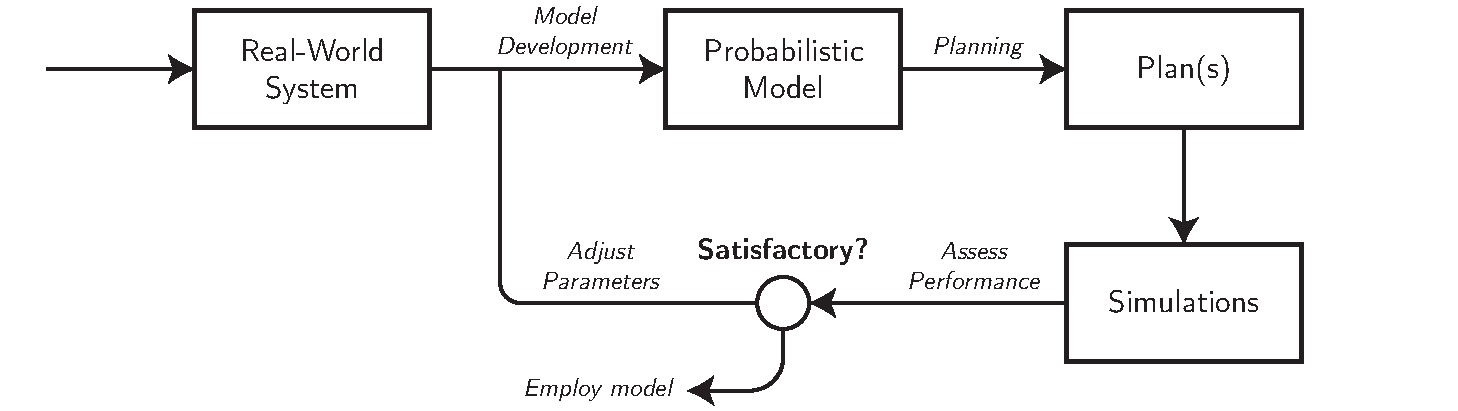
\includegraphics[width=\textwidth]{high-level-planning-diagram-cropped}
	\caption{Diagram showing a typical iterative procedure followed in the development of probabilistic models for planning under uncertainty. Given a problem description for the real-world system under consideration, a designer refines the model until satisfactory performance is observed.}
	\label{fig:high-level-model-development}
\end{figure}

The problem this thesis is concerned with is the development of probabilistic models, which are used for obtaining plans for automated control of systems whose dynamics are stochastic.
Setting up such models is an important, though difficult and time-costly process for a human designer that might not always have (enough) expertise to craft a suitable, well-generalizing model that can be used to plan for the execution of different tasks.
In practice, this problem is tackled by domain experts by iteratively tweaking the model parameters until the desired performance is achieved.
%The typical procedure is depicted in \autoref{fig:high-level-model-development} in which is seen that the model parameters are updated until satisfactory performance is observed.

\autoref{fig:high-level-model-development} shows a typical procedure followed in the design of a probabilistic model.
In this procedure, the human designer is presented a problem description and handcrafts an initial model for the system.
The model is then evaluated by performing tasks following the plans that are derived from the model in simulations or even in the real world.
The assessed performance steers the designer towards what model parameters appear to work well.
The designer uses the obtained knowledge to iteratively refine the model parameters until ultimately satisfactory performance is yielded in the execution of the derived plans.

An alternative that one ought to consider, is that of applying \acrshort{acr:rl} techniques rather than planning algorithms.
However, although ideas from planning and \acrshort{acr:rl} are interchangeable, these techniques typically demand direct interaction with the environment which is something that cannot always be readily offered.
That is, \acrshort{acr:rl} techniques turn out as time-consuming and sometimes even riskful or dangerous when applied in real-world environments.
Those domains for which plans need to be formulated offline, demand the acquisition of probabilistic models which accurately define what constitutes the state of the system, reflect uncertainty through transition probabilities and specify its goals in some manner.%TODO Rewrite 'some manner of specifying goals'?

An attractive approach of bypassing the daunting and error-prone task of handcrafting probabilistic models, is that of automatizing the model development process by applying learning algorithms on data that describes the dynamics of the system.
For this approach the data is typically presented in the form of execution traces of the system operating in a real-world environment, which is collected in an exploration phase prior to the actual planning.
However, although one could obtain a model of the system by applying learning algorithms, the corresponding plans that are inferred from this model might not be effective when applied in a real-world environment.
First of all, this might be due to the parameters of the learning algorithm not being set properly, signifying the need for proper adjustment of these parameters.
Another possibility is that the gathered data is incomplete and so does not accurately describe the dynamics of the system.
In this case, one could choose to augment the data for those areas for which the training data is inadequate, although one should be aware that this is accompanied by a more cost-expensive model-learning process.
Therefore, in order to learn accurate probabilistic models, we are in need of a way of assessing the performance of a model accompanied by a method for identifying inadequacies due to incomplete data, while taking into account the corresponding cost of learning and evaluating these system models.

\section{Research Questions}
\label{sec:research-questions}
The problem statement as presented in the previous section yields the following main research question for this thesis:

\vspace{12pt}
\noindent%\fbox{\parbox{\textwidth}{ %Uncomment this for boxes
\textbf{Main Research Question.} How can the task of obtaining a \acrfull{acr:mdp} that maximizes the yielded performance of executing plans that are derived from it, given a dataset about the system under consideration, be automated?
%}}
\vspace{12pt}

To answer this main research question, four research questions have been identified which are presented below.
The relevance of each of these research questions is discussed accordingly in the next paragraphs.

\vspace{16pt}
\noindent%\fbox{\parbox{\textwidth}{
\textbf{Research Question 1.} Which learning algorithms exist that can be employed for learning \acrshortpl{acr:mdp} from data for systems involving uncertainty that require plans for automated control?
%}}
\vspace{0pt}

First off, to facilitate the formulation of plans for a system involving uncertainty, we need to obtain an \acrshort{acr:mdp} from the provided dataset.
Therefore, we should know what learning algorithms exist that can be employed to learn the parameters of an \acrshort{acr:mdp}.
Accordingly, we should identify the applications for which each of these algorithms are suited, but also what the shortcomings or vulnerabilities of each of these algorithms are.

\vspace{16pt}
\noindent%\fbox{\parbox{\textwidth}{
\textbf{Research Question 2.} How should a performance measure be defined which can be used to fairly compare the value of different \acrshortpl{acr:mdp}?
%}}
\vspace{12pt}

As various \acrshortpl{acr:mdp} can be obtained for different parameter settings of the model learning algorithms, the need for a measure of performance for different \acrshortpl{acr:mdp} emerges.
That is, to establish which parameter settings yield an \acrshort{acr:mdp} that best reflects the underlying system for the tasks to be executed, we require a way to express and fairly compare the value of the learned \acrshortpl{acr:mdp}.

\vspace{16pt}
\noindent%\fbox{\parbox{\textwidth}{
\textbf{Research Question 3.} How can the parameter space of model learning algorithms cost-effectively be explored towards a global maximizer with only limited knowledge about the system under consideration?
%}}
\vspace{12pt}

A model learning algorithm may yield different \acrshortpl{acr:mdp} depending on the selected parameter settings.
To establish the most appropriate \acrshort{acr:mdp} for the system under consideration, the performance yielded by multiple \acrshortpl{acr:mdp} should be compared.
As evaluating all possible parameter-settings would be cost-expensive, we need to investigate other ways of exploring the parameter space more cost-effectively.
This is under the assumption that we only have limited to no belief over which parameter-settings might work well for the system under consideration.

\vspace{16pt}
\noindent%\fbox{\parbox{\textwidth}{
\textbf{Research Question 4.} How can the hierarchy of different abstraction levels be exploited to find a performance-maximizing \acrshort{acr:mdp} in a more cost-effective way?
%}}
\vspace{12pt}

Assessments of performance can be made at different levels of abstraction of the underlying system.
That is, we could examine how well an agent would perform a task only from the perspective of the \acrshort{acr:mdp} model, but also
from simulations or even the real world.
At the one hand abstracting from the real world typically yields a less accurate representation of the reality, although on the other hand assessing the performance from a more abstract level is accompanied by smaller computational costs.
Therefore, it might be valuable to investigate how this could be exploited to achieve a more cost-effective optimization of the performance.

%\vspace{12pt}
%\noindent\textbf{Research Questions:}
%\begin{enumerate}[label=\textbf{\arabic*})]
%	\item Which methods exist for learning (probabilistic) models from data for a system involving uncertainty that requires plans for automated control?
%	\item How should a performance measure be defined that can be used to fairly compare the value of different \acrshortpl{acr:mdp}?
%	\item How can the hierarchy of different abstraction levels be exploited to find a performance-maximizing \acrshort{acr:mdp} in a more cost-effective way?
%\end{enumerate}

\section{Contributions}
\label{sec:contribution}

We propose a framework for automating the development of probabilistic models in the form of \acrshortpl{acr:mdp} by applying learning algorithms on data describing the dynamics of the system under consideration.
The data about the environment that is used by these learning algorithms is gathered prior to the model learning process in an exploration phase.
%In order to obtain accurate probabilistic models for the system under consideration, the hyper-parameters of the used learning algorithm should be tweaked in such way to optimize the performance in the execution of its tasks.
Although various algorithms for learning \acrshortpl{acr:mdp} offline from a dataset \cite{shatkay1997learning, welch2003hidden, nikovski2002state} do already exist, the state of the art lacks a method for setting the hyper-parameters of these algorithms so to best reflect the underlying system and maximize the performance in the execution of its tasks.

%In order to obtain accurate probabilistic models for the system under consideration, the parameter-settings of the used model learning algorithm are iteratively tweaked towards a setting that maximizes the performance in the execution of the tasks expected to be performed.
%To achieve this we pose the adjustment of the learning algorithm parameters as an optimization task to maximize the performance that follows from executing plans derived from learned \acrshortpl{acr:mdp}.
To address this problem, the proposed framework poses the adjustment of the learning algorithm parameters as an optimization task of maximizing the performance that follows from executing plans derived from learned \acrshortpl{acr:mdp}.
The optimization is performed by applying a technique known as \acrfull{acr:bo}, such that we define a probability distribution over functions to model the performance measure and iteratively sample parameter-settings towards a global maximizer of the performance.
Although algorithms that employ the same framework for optimizing the parameters of probabilistic models \cite{ghavamzadeh2015bayesian, guez2012efficient} or policy search \cite{deisenroth2011pilco, wilson2014using} do exist, these are online approaches that do not utilise the available data prior to interacting with the real world environment.

%To address model inadequacies that are due to incomplete data, we propose to incorporate the identification of insufficient exploration for the transitions from those states that are visited in the execution of obtained plans.
%That is, for those learned models for which the data was observed to be incomplete, the observations of the performance for the corresponding parameter-settings are modeled as noisy or uncertain.
%This serves the purpose of more cautious exploitation of those areas of the parameter space which mostly produce noisy observations of the performance measure.

To achieve a more cost-effective optimization, the parameter search space is first narrowed down by a pre-processing step.
In this step assessments of the model value are made on a more abstract level (i.e., based on the computed value function for an \acrshort{acr:mdp}).
The posterior that follows from this step is then used to steer the acquisition in the main optimization step.

In attempt to further improve the learned models, a post-processing step is performed that aims to identify and fix discrepancies between the model and the real-world.
This post-processing step increases the resolution for those areas of the state-space when it identifies the outcomes of actions in simulations do not match the learned transition probabilities.

The framework is applied, tested and evaluated for the domain of mobile robot navigation, as the robots in this domain tend to operate under significant uncertainty in their actions.
A solution in this context is a policy which maps discretized robot poses into fine-grained navigation actions so to move a mobile robot to a certain goal location.
Probabilistic models are acquired by applying unsupervised machine learning algorithms on execution traces (consisting of odometry data describing robot poses) obtained in an exploration phase.
The optimization of the model is based on the performance of acquired models in simulations, which is expressed in terms of the time that has passed to reach multiple goal locations.
%Incomplete exploration data is here identified by inspecting the trajectories that are obtained from the execution of an optimal plan for an \acrshort{acr:mdp}.

% labeled as noisy uncertain observation of the performance of the model

% Discuss the learning and optimization routine: Automized method for learning probabilistic models in the form of MDPs by applying (machine) learning algorithms on exploration data. Optimization of the model by Bayesian Optimization based on performance in simulations.
% Identify incomplete exploration data about the environment by inspecting the observed trajectories and provide feedback on this from the optimization loop.
% Application to mobile robot navigation; A solution in this context is a policy that maps discretized robot poses into fine-grained navigation actions.

\section{Scope and Limitations}
\label{sec:scope-limitations}

First of all, we restrict ourselves to learning fully observable \acrshortpl{acr:mdp} from data.
However, this framework could possibly be extended to deal with applications where the states cannot be directly observed and should be inferred from observations.

Secondly, we note that all experiments and corresponding results are based on data that is solely obtained from simulations of a mobile robot.
Reasons for this are that we make the assumption that the environment is fully observable, which is typically not the case for real-world applications.
Another motivation of this is that the framework is not solely intended for the domain of mobile robot navigation and data from simulations is therefore deemed adequate for our experiments. % and not having a real robot at hand, which would be too expensive and comes with its own technical challenges that are outside of our scope.

Finally, we focus on the domain of mobile robot navigation to evaluate and test our approach.
One of the important aspects to consider, is which data should be collected to describe the dynamics of the system to learn models from this data.
For our implementation we choose to collect data about the robot's poses from internal odometry, but for other applications we might not be able to describe the states and transitions of the system through a geometric model and may need other learning algorithms than the clustering algorithms we use for our application.
An example of such applications might be that of learning \acrshortpl{acr:mdp} for traffic light control \cite{wiering2004intelligent, delgado2011efficient}, in which, for instance, lane-turn probabilities could be learned from a data-set.
Note that this application seems particularly appropriate to be approached in combination with \acrshort{acr:rl} techniques, so that the system is able to adapt to changes that occur over time.

% POMDPs: Restricted to MDPs, but could possible be extended to deal where the states are cannot be directly observed and should be inferred from observations.
% Field of application: We will discuss how the proposed method could be applied to other domains, although we will focus on the domain of mobile robot navigation to evaluate and test our method.

\section{Outline}
\label{sec:introduction-outline}

In this chapter we presented our motivations and defined the problem this thesis is concerned with.
To approach this problem we propose a framework that is aimed at automating the development of probabilistic models for the purpose of automated control by agents through planning under uncertainty.
This section describes the topics of the remaining chapters and how they relate to our problem statement and research questions presented earlier. % TODO Update

In \autoref{ch:background} we discuss the required background for both the planning and optimization aspect of this thesis.
First of all, in \autoref{sec:decision-theoretic-planning}, the chapter concretizes the type of problems dealt with in \acrshort{acr:dtp}. 
Accordingly, this chapter discusses the background on how dedicated probabilistic models can be used to reflect uncertainty in the systems under consideration.
It presents how these probabilistic models can be used by existing planning algorithms and how this relates to and differs from \acrshort{acr:rl} techniques.
Secondly, in \autoref{sec:bayesian-optimization}, the chapter discusses a method known as \acrlong{acr:bo} which we use for the optimization of the parameters of the model learning algorithms used in the proposed framework.
We formally describe how this method works and how it is applies to our problem of developing probabilistic models for planning, supported by a number of successful applications for learning and planning.
%For the optimization of the parameters of learning algorithms we use a method known as \acrlong{acr:bo}. In \autoref{ch:bayesian-optimization} we formally describe how this method works and how it is relevant to sequential decision making, supported by a number of successful applications for learning and planning.

In \autoref{ch:problem-related-work} we explore other existing techniques for the development of \acrshort{acr:mdp} models for systems involving uncertainty.
Apart from this we explore methods that takes advantage of techniques from the closely related field of \acrshort{acr:rl} to approach \acrshort{acr:sdm} problems where possible.
Additionally, the chapter reviews techniques that overcome the in-feasibility of accurately defining transition probabilities by accounting for uncertainty in these probabilities.

A solution to the problem we described, is proposed in \autoref{ch:methodology}, in which we put the theory and algorithms discussed in the earlier chapters together into an optimization routine.
%TODO Mention the running example

To test and evaluate our solution we choose to make an implementation for the optimization of probabilistic models for the path planning of a mobile robot.
In \autoref{ch:experimental-results} we discuss the results obtained from testing the proposed solution with our implementation for mobile robot navigation.

Finally, in \autoref{ch:conclusions} we summarize and evaluate the proposed solution. In this chapter we revisit our research questions and conclude this thesis with our recommendations and suggestions for future work.

%
%\vspace{12pt}
%\noindent\fbox{\textbf{TODO:} Needs small updates, in Contributions and the chapter overview}
%%